\subsubsection{UCA 6 - Tracciamento posizione in un luogo di un'organizzazione}%kite level

\begin{figure}[h]
	\centering
	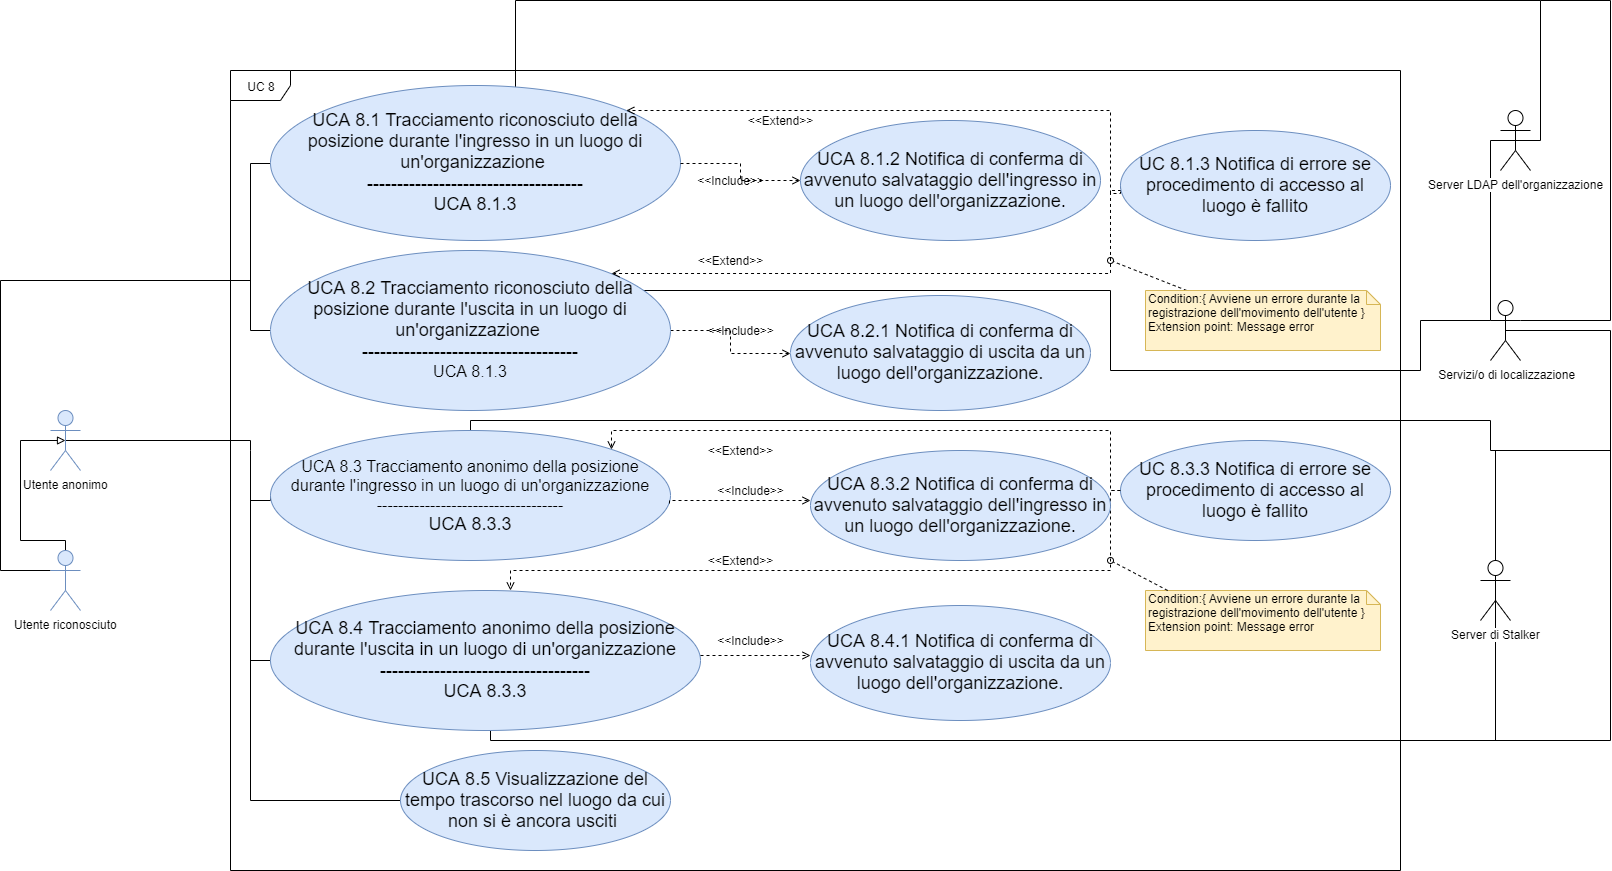
\includegraphics[scale=0.3]{sezioni/UseCase/Immagini/UCA6.png}
	\caption{Tracciamento\ap{G} posizione in un luogo di un'organizzazione\ap{G}}
\end{figure}

\begin{itemize}
	\item \textbf{Attori primari:} Utente anonimo, Utente riconosciuto
	\item \textbf{Attori secondari:} Servizi/o di localizzazione (GPS\ap{G}, rete cellulare).
	\item \textbf{Precondizione:} L'utente autenticato\ap{G} con credenziali Stalker sta per effettuare un movimento\ap{G} in un luogo dell'organizzazione\ap{G} che richiede il tracciamento\ap{G}.
	\item \textbf{Postcondizione:} Viene memorizzato dal sistema: il timestamp\ap{G}, i momenti in cui è avvenuto il tracciamento \ap{G}, dove è avvenuto e il tempo trascorso al suo interno.
	\item \textbf{Scenario principale:} L'utente si trova nei pressi o sta per uscire da un luogo dell'organizzazione\ap{G} che richiede il tracciamento\ap{G}. Viene salvato il timestamp\ap{G} di entrata ed uscita dall'organizzazione\ap{G} e viene salvato il tempo trascorso all'interno dell'organizzazione\ap{G}. L'utente riceve inoltre una notifica per l'entrata e l'uscita dall'organizzazione.
\end{itemize}

\begin{figure}[h]
	\centering
	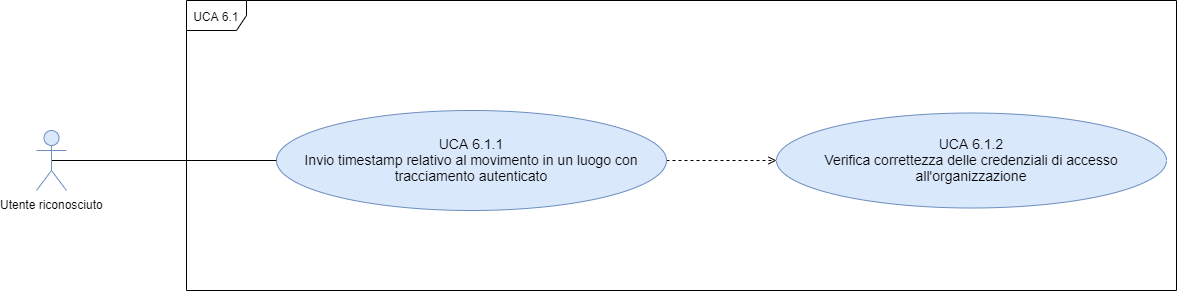
\includegraphics[scale=0.4]{sezioni/UseCase/Immagini/UCA6.1.png}
	\caption{Tracciamento\ap{G} autenticato della posizione durante l'ingresso in un luogo di un'organizzazione\ap{G}}
\end{figure}
\subsubsection{UCA 6.1 - Tracciamento autenticato della posizione durante l'ingresso in un luogo di un'organizzazione}
\begin{itemize}
	\item \textbf{Attori primari:} Utente riconosciuto
	\item \textbf{Attori secondari:} Servizi/o di localizzazione (GPS\ap{G}, rete cellulare), server LDAP\ap{G} dell'organizzazione.
	\item \textbf{Precondizione:} L'utente sta per entrare (ovvero si trova nei pressi) in un luogo dell'organizzazione\ap{G} che richiede il tracciamento autenticato\ap{G}.
	\item \textbf{Postcondizione:} Viene registrato l'ingresso nel luogo dell'organizzazione\ap{G} in una certa data e ora (timestamp\ap{G}).
	\item \textbf{Scenario principale:} L'utente entra nel luogo dell'organizzazione\ap{G}, tramite i/il servizio/i di localizzazione, viene salvato e notificato tale ingresso.
	\item \textbf{Flusso di eventi:}
	\begin{enumerate}
		\item l'utente accede nel luogo dell'organizzazione\ap{G};
		\item Viene inviato il timestamp \ap{G} del ingresso [UCA 6.1.1];
		\item Vengono verificate le credenziali dell'utente [UCA 6.1.2];
		\item Viene informato l'utente che è stato memorizzato il suo ingresso nel luogo\ap{G}.
	\end{enumerate}
	\item \textbf{Scenario alternativo:} Il tentativo di autenticazione\ap{G} presso l'organizzazione\ap{G} o l'invio delle credenziali fallisce. Viene informato l'utente.
	\item \textbf{Estensioni:}
	\begin{enumerate}
		\item UCA 7.6.1 - Notifica di errore se procedimento di memorizzazione del movimento al luogo è fallito.
	\end{enumerate}
	\item \textbf{Inclusioni:}
	\begin{enumerate}
		\item UCA 6.1.3 - Notifica di avvenuta memorizzazione dei dati del movimento.
	\end{enumerate}
\end{itemize}

\subsubsection{UCA 6.1.1 - Invio timestamp relativo al movimento in un luogo con tracciamento autenticato}
\begin{itemize}
	\item \textbf{Attori primari:} Utente riconosciuto
	\item \textbf{Precondizione:} L'utente ha effettuato un movimento\ap{G} in un luogo\ap{G} che richiede il tracciamento autenticato\ap{G}.
	\item \textbf{Postcondizione:} Viene registrato il timestamp\ap{G} relativo a un movimento\ap{G} effettuato nel luogo dell'organizzazione\ap{G}.
	\item \textbf{Flusso di eventi:}
		\begin{enumerate}
			\item viene in inviato il timestamp\ap{G} relativo al movimento\ap{G} dell'utente;
			\item vengono verificate le credenziali di accesso [UCA 6.1.2];
			\item vengono registrate la informazioni relative alla data e ora del movimento\ap{G} fatto dall'utente.
		\end{enumerate}
	\item \textbf{Inclusioni:}
		\begin{itemize}
			\item UCA 6.1.2 - Verifica correttezza delle credenziali di accesso all'organizzazione.
		\end{itemize}
\end{itemize}

\subsubsection{UCA 6.1.2 - Verifica correttezza delle credenziali di accesso all'organizzazione}
\begin{itemize}
	\item \textbf{Attori primari:} Utente riconosciuto
	\item \textbf{Attori secondari:} Server\ap{G} dell'organizzazione.
	\item \textbf{Precondizione:} L'utente, in quanto riconosciuto, possiede credenziali per autenticarsi presso l'organizzazione \ap{G}.
	\item \textbf{Postcondizione:} Viene verificato che le credenziali fornite sono valide.
\end{itemize}

\subsubsection{UCA 6.1.3 - Notifica di avvenuta memorizzazione dei dati del movimento}
\begin{itemize}
	\item \textbf{Attori primari:} Utente riconosciuto, Utente anonimo
	\item \textbf{Precondizione:} Il processo di memorizzazione dei dati del movimento\ap{G} nel sistema è avvenuto correttamente.
	\item \textbf{Postcondizione:} Viene notificato l'utente dell'avvenuto salvataggio.
\end{itemize}

\begin{figure}[h]
	\centering
	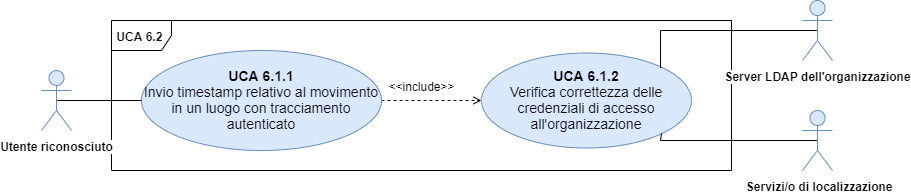
\includegraphics[scale=0.4]{sezioni/UseCase/Immagini/UCA6.2.png}
	\caption{Tracciamento\ap{G} autenticato della posizione durante l'uscita in un luogo da un'organizzazione\ap{G}}
\end{figure} 

\subsubsection{UCA 6.2 - Tracciamento autenticato della posizione durante l'uscita da un luogo di un'organizzazione}
\begin{itemize}
	\item \textbf{Attori primari:} Utente riconosciuto
	\item \textbf{Attori secondari:} Servizi/o di localizzazione (GPS\ap{G}, rete cellulare), server LDAP\ap{G} dell'organizzazione.
	\item \textbf{Precondizione:} L'utente sta per uscire da un luogo dell'organizzazione\ap{G} che richiede il tracciamento\ap{G}.
	\item \textbf{Postcondizione:} Viene registrata l'uscita dal luogo dell'organizzazione\ap{G} in una certa data e ora (timestamp\ap{G}).
	\item \textbf{Scenario principale:} L'utente esce dal luogo dell'organizzazione\ap{G}, tramite i/il servizio/i di localizzazione, viene salvato e notificato tale uscita\ap{G}. 
		\item \textbf{Flusso di eventi:}
	\begin{enumerate}
		\item l'utente esce dal luogo dell'organizzazione\ap{G};
		\item Viene inviato il timestamp \ap{G} del uscita [UCA 6.1.1];
		\item Vengono verificate le credenziali dell'utente [UCA 6.1.2];
		\item Viene informato l'utente che è stata memorizzata la sua uscita dal luogo\ap{G} [UCA 6.1.3].
	\end{enumerate}
	\item \textbf{Scenario alternativo:} Il tentativo di autenticazione\ap{G} presso l'organizzazione\ap{G} o l'invio delle credenziali fallisce. Viene informato l'utente.
	\item \textbf{Estensioni:}
		\begin{enumerate}
		\item UCA 7.6.1 - Notifica di errore se procedimento di memorizzazione del movimento al luogo è fallito.
	\end{enumerate}
	\item \textbf{Inclusioni:}
	\begin{enumerate}
		\item UCA 6.1.3 - Notifica di avvenuta memorizzazione dei dati del movimento.
	\end{enumerate}
\end{itemize}

\subsubsection{UCA 6.3 - Tracciamento anonimo della posizione durante l'ingresso in un luogo di un'organizzazione}
\begin{itemize}
	\item \textbf{Attori primari:} Utente anonimo
	\item \textbf{Attori secondari:} Servizi/o di localizzazione (GPS\ap{G}, rete cellulare)
	\item \textbf{Precondizione:} L'utente sta per entrare (ovvero si trova nei pressi) in un luogo dell'organizzazione\ap{G} che richiede il tracciamento anonimo\ap{G}.
	\item \textbf{Postcondizione:} Viene registrato l'ingresso nel luogo dell'organizzazione\ap{G} in una certa data e ora (timestamp\ap{G}).
	\item \textbf{Scenario principale:} L'utente entra nel luogo dell'organizzazione\ap{G}, tramite i/il servizio/i di localizzazione, viene salvato e notificato tale ingresso.
	\item \textbf{Flusso di eventi:}
	\begin{enumerate}
		\item l'utente accede nel luogo dell'organizzazione\ap{G};
		\item Viene inviato il timestamp \ap{G} del ingresso [UCA 6.3.1];
		\item Viene informato l'utente che è stato memorizzato il suo ingresso nel luogo\ap{G}.
	\end{enumerate}
	\item \textbf{Scenario alternativo:} L'invio delle credenziali fallisce. Viene informato l'utente.
	\item \textbf{Estensioni:}
	\begin{enumerate}
		\item UCA 7.6.1 - Notifica di errore se procedimento di memorizzazione del movimento al luogo è fallito.
	\end{enumerate}
	\item \textbf{Inclusioni:}
	\begin{enumerate}
		\item UCA 6.1.3 - Notifica di avvenuta memorizzazione dei dati del movimento.
	\end{enumerate}
\end{itemize}

\subsubsection{UCA 6.3.1 - Invio timestamp relativo al movimento in un luogo con tracciamento anonimo}
\begin{itemize}
	\item \textbf{Attori primari:} Utente anonimo
	\item \textbf{Precondizione:} L'utente ha effettuato un movimento\ap{G} in un luogo\ap{G} che richiede il tracciamento anonimo\ap{G}.
	\item \textbf{Postcondizione:} Viene registrato il timestamp\ap{G} relativo a un movimento\ap{G} effettuato nel luogo dell'organizzazione\ap{G}.
	\item \textbf{Flusso di eventi:}
	\begin{enumerate}
		\item viene in inviato il timestamp\ap{G} relativo al movimento\ap{G} dell'utente;
		\item vengono registrate la informazioni relative alla data e ora del movimento\ap{G} fatto dall'utente.
	\end{enumerate}
\end{itemize}

\subsubsection{UCA 6.4 - Tracciamento anonimo della posizione durante l'uscita in un luogo di un'organizzazione}
\begin{itemize}
	\item \textbf{Attori primari:} Utente anonimo
	\item \textbf{Attori secondari:} Servizi/o di localizzazione (GPS\ap{G}, rete cellulare)
	\item \textbf{Precondizione:} L'utente sta per uscire da un luogo dell'organizzazione\ap{G} che richiede il tracciamento\ap{G}.
	\item \textbf{Postcondizione:} Viene registrata l'uscita dal luogo dell'organizzazione\ap{G} in una certa data e ora (timestamp\ap{G}).
	\item \textbf{Scenario principale:} L'utente esce dal luogo dell'organizzazione\ap{G}, tramite i/il servizio/i di localizzazione, viene salvato e notificato tale uscita\ap{G}. 
	\item \textbf{Flusso di eventi:}
	\begin{enumerate}
		\item l'utente esce dal luogo dell'organizzazione\ap{G};
		\item Viene inviato il timestamp \ap{G} del uscita [UCA 6.3.1];
		\item Viene informato l'utente che è stata memorizzata la sua uscita dal luogo\ap{G} [UCA 6.1.3].
	\end{enumerate}
	\item \textbf{Scenario alternativo:} L'invio delle credenziali fallisce. Viene informato l'utente.
	\item \textbf{Estensioni:}
	\begin{enumerate}
		\item UCA 7.6.1 - Notifica di errore se procedimento di memorizzazione del movimento al luogo è fallito.
	\end{enumerate}
	\item \textbf{Inclusioni:}
	\begin{enumerate}
		\item UCA 6.1.3 - Notifica di avvenuta memorizzazione dei dati del movimento.
	\end{enumerate}
\end{itemize}